\documentclass{article}
\usepackage{tikz}

\usetikzlibrary{arrows,decorations.markings}

\title{Political Science 101 notes}
\author{Conrad A. Mearns}

\begin{document}

\maketitle

\noindent
\Large Quotes\\\\
\normalsize
\quote{A nation that hates politics will not long survive as a democracy.} - E. J. Dionne

\noindent
\Large January 11, 2017\\\\
What is Political Science?
\normalsize

\noindent
Politics is "Who gets what, when and how?" It is the resolution of peaceful conflict or rare and scarce things.
\begin{itemize}
  \item Who --- parties, individuals, citizens, instututions
  \item What --- money, distrubution, rights, symbolism
  \item Where and How --- congressional legistlation, court, executive order, voting
\end{itemize}

\noindent
There are three kinds of statements to be made in Political Science
\begin{itemize}
  \item Descriptive --- True / False --- things that can be perceieved --- "It is snowing"
  \item Evaluative --- Good / Bad --- normative, defines morals --- "It is good that there are 100 senators"
  \item Explanatory --- Cause / Effect --- why do people vote the way they do? Ways to relate variables. --- "Trump was elected with help of foreign interference"
\end{itemize}

\noindent
It is important to differentiate cause from correlation. Post hoc ergo propter hoc --- After this, therefor because of this. It was winter, now it is spring. Therefor winter caused spring.

\noindent
Democracy can adapt. Policy that affects a majority can only be enacted with support from that majority.\\

\noindent
\Large January 13, 2017\\\\
On Reading Sources\\
\normalsize
\noindent
Arguement - A set of proposition to lead us to a conclusion.

\begin{enumerate}
  \item Consider the source
  \item Lay out the arguement
  \item Find evidence and claims to support propositions
  \item Evaluate the conclusion
  \item Consider the consequences or purpose
\end{enumerate}

\noindent
\Large On Power and Authority\\
\normalsize
\noindent
Suppose people-entities $A$ and $B$.

\centering
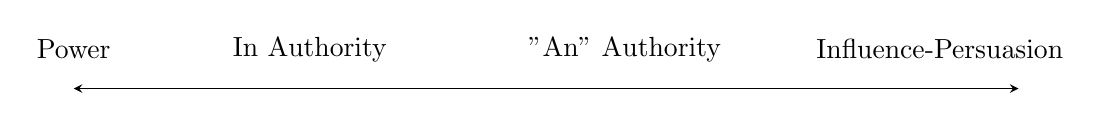
\begin{tikzpicture}
  \node (a) at (0,1) {Power};
  \node (b) at (3,1) {In Authority};
  \node (c) at (7,1) {"An" Authority};
  \node (d) at (11,1) {Influence-Persuasion};
  \draw [<->,>=stealth] (0,.5) -- (12,.5);
\end{tikzpicture}
\raggedright

\begin{itemize}
  \item Power: $A$ creates a threat to force $B$ to conform to what $A$ wants. Either by taking benifits or imposing punishment.
  \item In Authority: Power is possibly given to $A$ to threaten $B$ into doing what $A$ wants.
  \item "An" Authority: $A$ suggest $B$ to take some form of action because it benifits $B$, only because $B$ looks up to $A$.
  \item Influence-Persuassion: $A$ wants something so $A$ persuades $B$ to conform for the self interest of $B$.
\end{itemize}

\noindent
Authority is an assignment of resources of power given to a holder when needed. It does not promise control, only access or oppurtunity to power.

\Large On Defining Democracy\\
\normalsize
\noindent
See James Madison's Federalist Paper 10.\\

"Democracy" has it's roots from the Greek words d\={e}mos and -kratia, meaning "the people" and "power / rule" respectively. The democracy we know isn't the Athenian democracy originially idealized, it's actually a Republic. Athenian democracy is centered around what's popular, and participation. That is to say, Athenian democracy requires more than just voting on ideas, it requires deliberation and constant confliction. People who follow this belief are Popular Democrats.\\

Elite Democrats are the proposed solution by James Madison. He argued that humans are, by nature, private and passionate. By forming groups, we try to impose our beliefs guided by emotion and passion - self interest. Elite Democrats are to be commited to formality and compomise for the percieved greater good of everyone affected.

\end{document}
